In cui si descrive la progettazione del software: scelte progettuali, tecnologie e linguaggi adottati.

\section{Gerarchia degli utenti}
Si è scelto per la gerarchia a tre livelli \ref{3-level}, lasciando la gerarchia a quattro livelli \ref{4-level} come futuro sviluppo, essendo una semplice estensione della prima possibilità.

\section{Greenbone OpenVAS}
Come backend di scansione per il sistema, inizialmente si è optato per interfacciarsi a \textbf{Greenbone OpenVAS}.

\subsection{Storia del progetto}
\textbf{OpenVAS} (\emph{Open Vulnerability Assessment Scanner}) è una piattaforma \emph{open source} per la rilevazione, l'analisi e la gestione di vulnerabilità e falle di sicurezza.

OpenVAS Nasce nel 2005 come \emph{fork} dello scanner \textbf{Nessus}, quando questi modificò la propria licenza, diventando da \emph{open source} un software proprietario distribuito sotto licenza commerciale. La comunità open source da quel momento ha manutenuto il fork risultante, inizialmente denominato \emph{GNessUs} e poi rinominato in \emph{OpenVAS}. Tempo dopo entrò a far parte dei progetti supportati economicamente dalla \emph{Software in the Public Interest}.

Tra i principali contributori del fork vi erano gli sviluppatori di Intevation e DN-Systems, aziende che poi sarebbero diventate Greenbone AG e finanziate dalla BSI tedesca (l'Ufficio Federale per la Sicurezza Informatica). Eventualmente nel 2008 la neo-costituita Greenbone si propose tra gli obiettivi aziendali il sostenere lo sviluppo open source di OpenVAS e creare delle versioni maggiormente supportate e curate per i clienti enterprise, oltre all'offrire il necessario supporto. Oltre a Greenbone, con il tempo si unirono al progetto altre aziende per contribuire eventualmente ad un feed stabile e aggiornato di test di vulnerabilità, componente chiave ed essenziale dell'intero progetto.

Eventualmente già nel 2010 OpenVAS ruppe la compatibilità con Nessus e negli anni successivi ricevette ulteriore supporto dalla BSI e anche dalla DFN (la rete di ricerca tedesca usata da università e centri di ricerca), nella forma di avvisi di sicurezza regolari pubblicati sotto licenza GPL.

Nel 2017 i contributi di Greenbone diventarono palesi con un cambio di nome ufficiale: il progetto non si sarebbe più chiamato \emph{OpenVAS framework}, ma \textbf{Greenbone Vulnerability Management (GVM)}, un framework completo di sicurezza informatica, dove per OpenVAS si intende solo lo scanner vero e proprio, uno dei tanti componenti.

\subsection{Modello di business}
Greenbone OpenVAS e GVM possono ricevere gli aggiornamenti di sicurezza e configurazioni da due feed, entrambi manutenuti da Greenbone:
\begin{itemize}
    \item \textbf{Greenbone Community Feed}: questo canale di aggiornamenti è totalmente gratuito e open-source. Contiene versioni minimali e preconfigurate di configurazioni di scansione, liste di porte, reportistica; ma soprattutto, in questo feed non sono incluse tutti i test di vulnerabilità disponibili, limitandosi a fornire esclusivamente quelli più critici e importanti. I dati sono aggiornati giornalmente secondo una policy di best effort e senza garanzie di alcun tipo.
    \item \textbf{Greenbone Enterprise Feed}: questo canale di aggiornamenti è invece a pagamento, ed è pensato per i clienti di Greenbone che usano il framework GVM in contesti aziendali. In questo canale sono forniti tutti i test di vulnerabilità disponibili, ma anche tutte le configurazioni di scansione e reportistica. Il servizio è inoltre garantito sotto SLA\footnote{\emph{Service Level Agreement}: contratto in cui un provider di un servizio garantisce agli utenti di quel servizio degli standard minimi di qualità e disponibilità.}
\end{itemize}
Il progetto è sostenuto economicamente soprattutto attraverso la sottoscrizione al secondo feed da parte dei clienti di tipo \emph{enterprise}. In aggiunta, Greenbone fornisce anche \emph{hardware appliance}\footnote{Dispositivi fisici progettati per eseguire una specifica funzione / applicazione, ottimizzati espressamente per quell'unico scopo.}, \emph{virtual appliance}\footnote{Sistemi informatici virtuali che eseguono una specifica funzione / applicazione, progettati per essere installati e usati in un software di virtualizzazione.} e una soluzione SaaS gestita direttamente da loro.

\subsection{Architettura}
L'architettura del framework Greenbone Vulnerability Management (GVM) è organizzata nei seguenti raggruppamenti:
\begin{itemize}
    \item Applicazioni eseguibili per lo scanner e lo scanner stesso, tutti con lo scopo comune di eseguire \textbf{Vulnerability Test (VT)} sui sistemi bersaglio.
\end{itemize}

\begin{figure}
    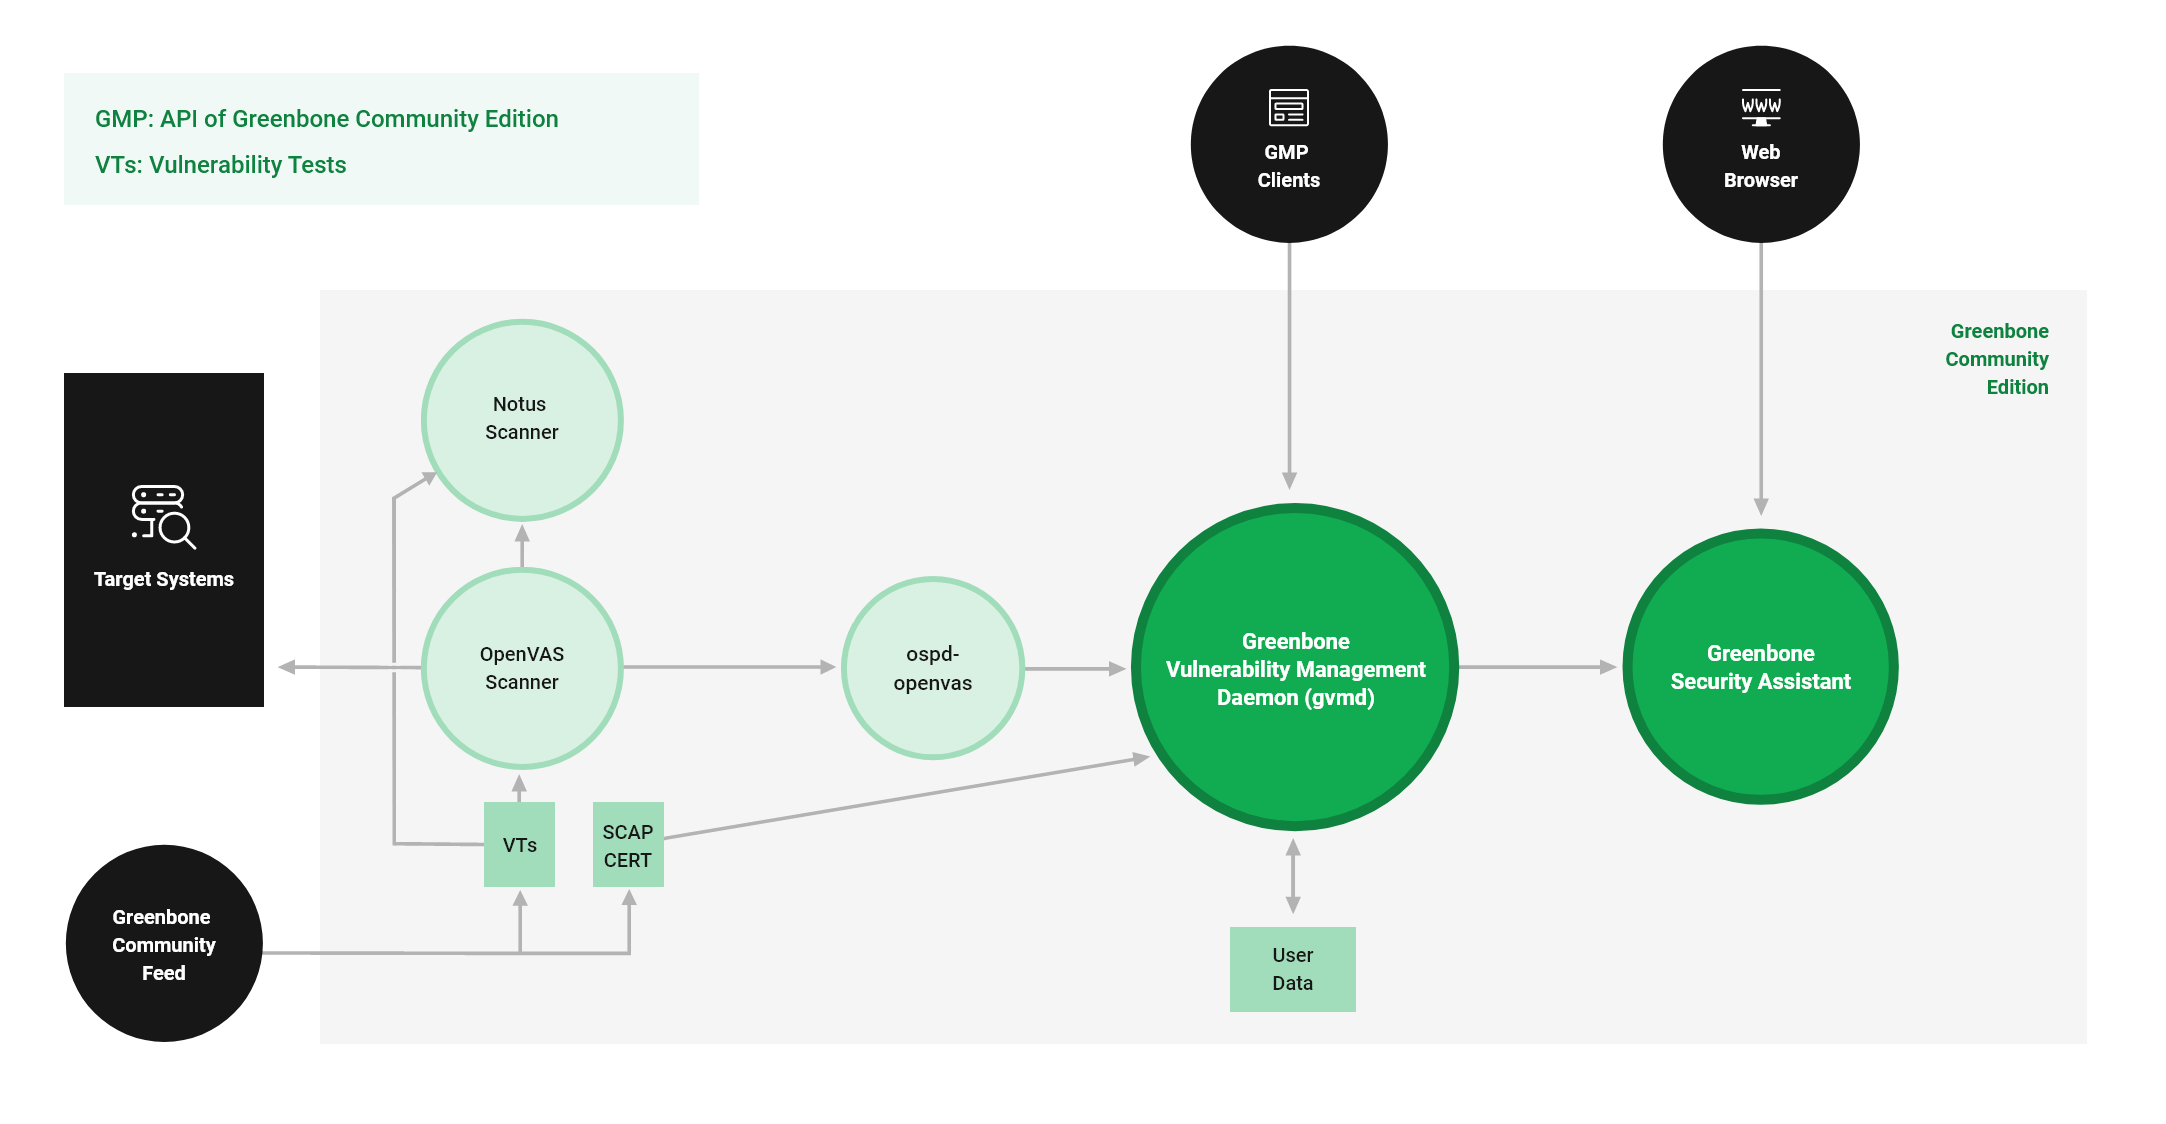
\includegraphics[width=\textwidth]{img/greenbone-community-22.4-architecture.png}
    \caption{Architettura della release 22.4 (ultima al momento della stesura del documento)}
\end{figure}


\subsection{Motivazioni alla base della scelta}
I principali motivi alla base di questa scelta sono:
\begin{itemize}
    \item \textbf{Disponibilità di una versione gratuita}: OpenVAS può essere installato e amministrato direttamente dall'azienda senza costi di licenze o abbonamenti, preoccupandosi solo di predisporre e manutenere l'hardware necessario.
    
    Tuttavia, è importante far notare ancora una volta come la versione gratuita di OpenVAS non disponga di tutti i test di sicurezza disponibili, rendendo necessaria un'ulteriore analisi per verificare se i dati forniti siano sufficienti agli scopi aziendali.

    \item \textbf{Open source}: OpenVAS è open source, perciò il suo codice è liberamente visibile se necessario, evitando durante lo sviluppo il rischio di incorrere in componenti non documentati o comunque opachi.
    
    \item \textbf{Librerie ufficiali}: inoltre, Greenbone mantiene anche degli strumenti ufficiali per interfacciarsi con il sistema OpenVAS, tra cui soprattutto una libreria Python che cerca di implementare quante più funzionalità del protocollo GMP.
\end{itemize}